\section{Loop Optimizations}
\subsection{Loop in CFG}
循环在控制流图(CFG)体现为 一个节点集合 $S$, 包含 header node $h$, 并且对于 $S$ 中的任何节点 $x$:
\begin{itemize}
    \item 都有一条从 $x$ 到 $h$ 的路径
    \item 都有一条从 $h$ 到 $x$ 的路径
    \item 除了 $h$, 没有任何其他 $S$ 以外的节点能到达 $x$
\end{itemize}

\subsubsection{Dominator tree}
重要概念:
\begin{itemize}
    \item Loop entry: $h$ 是唯一一个能从外部到达的节点, 是循环的唯一入口
    \item Loop exit: 可以有多个节点能跳出循环(i.e. 后继节点不都属于 $S$)
    \item Predecessor: pred, 前驱节点
    \item Successor: succ, 后继节点
    \item Dominator: 如果 CFG 的入口节点 $s_0$ 到节点 $n$ 的所有路径都经过节点 $d$, 我们就称 $d$ 是 $n$ 的支配节点(dominator), 记作 $d \dom n$. 
    \subitem 每个节点都支配(dominate)自己
    \subitem 节点可以有多个 dominators
    % \begin{figure}[H]
    %     \centering
    %     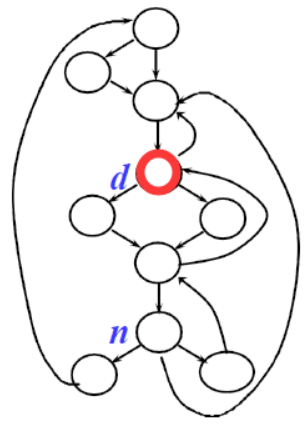
\includegraphics[width=0.3\linewidth]{pic/CP18/dominator}
    %     \caption{dominator}
    % \end{figure}
    \subitem 求解每个节点的 dominators $D[n]$:
    \begin{itemize}
        \item 入口节点的 dominator 就是自己: $D[s_0]=\{ s_0 \}$
        \item 对于其它节点: 
        \begin{align*}
            D[n]=n\cup \left( \bigcap_{p\in pred[n]} D[p] \right) \text{ for }n\ne s_0
        \end{align*}
        \item 求解过程: 一开始时令 $D[s_0]=\{ s_0 \}$, 其余节点 $D[x]=$所有节点; 然后使用上面的式子不断迭代更新直到不动点. 
    \end{itemize}
    \item Immediate dominator: 直接支配节点, 支配 $n$ 的节点中距离 $n$ 最近(但不是自己)的节点. 
    \subitem 也就是从入口结点到达 $n$ 的任何路径(不含 $n$) 中, 路径中最后一个支配 $n$ 的结点. 
    \subitem $n$ 的直接支配节点记作 $idom(n)$.
    \subitem 除了初始节点 $s_0$ 以外, 每个节点有且仅有一个直接支配节点. 
    \item Dominator tree: 支配节点树
    \subitem 对于每个节点 $n$, 连接边: $idom(n)\to n$.
    \subitem 每个节点支配以自己为根的子树中的所有节点
    \begin{figure}[H]
        \centering
        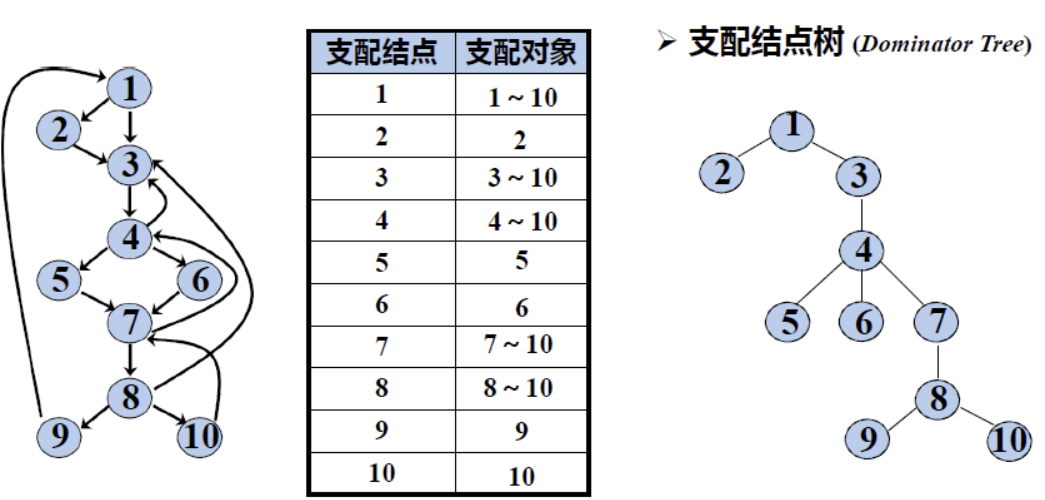
\includegraphics[width=0.84\linewidth]{pic/CP18/Dominator tree}
        \caption{Dominator tree}
    \end{figure}
\end{itemize}

\subsubsection{Natural Loop}
自然循环. 并不关心循环具体代码形式, 而是关心能否提取出易于优化的循环结构. 

如果边 $n\to h$ 满足 $h \dom n$, 则这是一个 back edge. Back edge 指向的节点 $h$ 称为 loop header.

可以基于 back edge 严谨地定义 CFG 图中的一个自然循环: 
\begin{definition}
    每个 back edge $n\to h$ 对应一个 natural loop. 这个 natural loop 中的节点集合包含一些节点 $x$ 满足: 
\begin{itemize}
    \item $h \dom x$
    \item 存在一条从 $x$ 到 $n$ 的路径不经过 $h$. 
\end{itemize}
\end{definition}
说人话就是 back edge 是从循环尾回到循环头(loop header)的边; 循环体就是中间那些被 loop header 支配的节点.  而 back edge 的意义是保证至少有一条路径能返回首节点 $h$. 

可以有多个 back edge 对应一个 natural loop: 例如 for 语句中的每个 continue 都给这个 natural loop 新增了一个 back edge.

注:
\begin{itemize}
    \item 循环可以嵌套, 可以共享首节点.
    \item 除了共享首节点的情况外, 两个循环要么完全不相交, 要么一个完全嵌入另一个(或者说后者包含前者). 
    \item 最内循环(innermost loop): 最里的循环, 不包含其他循环(不被其他循环嵌入). 
\end{itemize}


\subsubsection{Loop-nest Tree}
表达循环的嵌套关系. 树中每个节点对应一个 loop header 及其对应的 natural loops 节点集合. 如果这个 loop heder 对应多个 natural loops (共享首节点), 也合并到同一个节点. 

\begin{figure}[H]
    \centering
    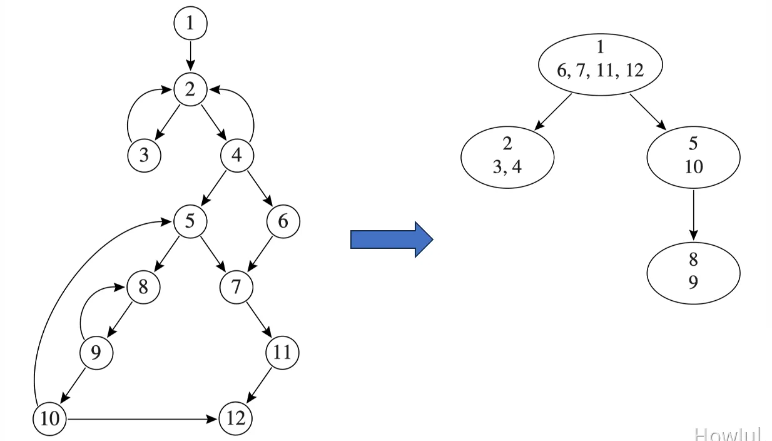
\includegraphics[width=0.84\linewidth]{pic/CP18/Loop-nest Tree}
    \caption{Loop-nest Tree}
\end{figure}
节点的上半部分表示该节点对应的 loop header. 可以把整个 procedure 视为在一个假想的大循环中, 作为树的根节点. 叶节点即对应最内循环. 

Loop preheader: 前置首节点. 许多优化操作会在进入循环前进行一些准备工作, 也就是在紧挨着循环头之前插入一些语句. 因此我们可以在 loop header 之前插入一个 loop preheader 用来安置这些语句. 
\begin{itemize}
    \item loop preheader 的唯一后继就是 loop header
    \item 循环 $L$ 外到达首节点的边 $x\to h$ 改为进入前置首节点: $x\to p$
    \item 循环 $L$ 里到达首节点的边不变
\end{itemize}

\subsection{Loop Invariant Hoisting}
循环不变代码外提.

Loop-invariant: 如果某个表达式的值在循环中不会改变, 对循环来讲是固定值, 则称表达式 loop-invariant. 显然, 所有常数都 loop-invariant. 

赋值语句 $x := v_1\text{ OP }v_2$  是 invariant 的当且仅当其操作数 $v_1$ 和 $v_2$ 都满足: 
\begin{itemize}
    \item 操作数是常数, 或是
    \item 对于操作数中使用到的变量, 其 def 都在循环外, 或是
    \item 对于操作数中使用到的变量, 在执行赋值语句时其 def 唯一, 且 loop-invariant.
\end{itemize}
说人话就是操作数及其使用的变量也得 loop-invariant, 而且不能在循环中因为控制流跳转等原因导致变量 def 不唯一. 


可以归纳地检查赋值语句 $x := v_1\text{ OP }v_2$ 的操作数是否 invariant:
\begin{itemize}
    \item Base cases:
    \subitem 常数: 一定是 invariant 的. 
    \subitem 变量的 use: 该变量所有 defs 都在循环外则 invariant.
    \item Inductive cases:
    \subitem 表达式: 多个 invariant 表达式进行运算仍然 invariant.
    \subitem 变量的 use: 要求在执行该语句时只可能有唯一的 def 有效, 且这个 def 的右侧(RHS) 是 loop-invariant 的. 
\end{itemize}

优化: 这样的表达式在循环外就可以求值, 而非每轮循环都计算一次. 这就是 loop-invariant code motion.
\begin{itemize}
    \item Code hoisting: 如果这样的表达式在循环中需要使用, 则可以将求值提升到循环开始前. 
    \item Code sinking: 如果这样的表达式在循环结束后需要使用, 则可以将求值下沉到循环结束后. 
\end{itemize}

注意表达式的值是 loop-invariant 的不代表 hoisting 就是合法的: 归根结底, 这相当于只关心了 表达式 的值, 但忽视了其副作用; 盲目上提会破坏代码的语义(semantics)信息. 

\subsubsection{Code hoisting}
hoisting 的判据: 当且仅当满足如下所有条件时可以提升形如 $t := a\text{ OP }b$ 的赋值语句(赋值语句就是 def)$d$:
\begin{itemize}
    \item $d$ 必须支配所有 $t$ 在其上 live-out 的循环出口(loop exits).
    \item 在循环中 $t$ 只能有唯一的 def.
    \item $t$ 不属于 loop preheader 的 live-out 集合; 换句话说, $t$ 在进入循环前不是活跃的. 
\end{itemize}

如果这个赋值语句有一定的副作用, 那么上述规则就不足够, 需要添加更多判断、约束. 

将 while 转写为 for 有助于优化: 拷贝一份条件判断块到循环体末尾即可. 这是由于 while 特殊的控制流结构可能会导致判据中最后一条要求无人能达到, 要把 while 转化为刚刚研究的 repeat-until 这种模式的 natural loops.